\documentclass[twocolumn]{article}
\usepackage{graphicx}

\begin{document}
\title{Homework 7: Round-trip time measurements - Playing around with Planetlab}
\author{Raghavan KL}
\maketitle

\begin{abstract}
In this homework, I measure and report  round-trip times for 200 Planetlab hosts. I have used these planet lab machines to ping each other and collected their data, based on this data I have made estimations on rtt and distance between the machines around the world. Following are the steps involved and they are explained in detail in this document,

\begin{itemize}
\item Collection of data
\item Extraction/Cleaning
\item Visualization of data
\item Analysis
\item Inference
\end{itemize}

The whole process was carried out in two different time intervals one was on \textit{Nov-12-2012 10.00PM(Night)} and other was on \textit{Nov-13-2012 9.00AM(Morning)}.

\end{abstract}


\section{Collection}
After getting a planet lab account, I was able to login to any of the active planet machines(approx. 200).Then I passed a file to all the planet lab machine which consist of ping command to all machines. The ping data of all these machines I extracted and placed into my local log file. This step was optimized by running the commands in the background instead of waiting in the foreground, by this I managed to gather around 300,000 ping records. The distance between every other IP is calculated using the perl library which manipulates them based on the lattitude, longitude of IPs. A total record set of 200 * 200 IPs is calculated in the format of \textbf{\textit{From IP, To IP, Distance}} and stored for future use. One time storage of this data would be a viable idea since this would be a static data and no need to calculate them again.

\section{Extraction/Cleaning}

\subsection{Extracting ping data}
The ping data which is gathered is then structured into a file consisting of the format  \textbf{\textit{From IP, To IP, RTT Time}}. This is an cleaned dataset derived out the whole ping dataset which was gathered during the collection process.

\subsection{Merging distance and Ping dataset}
The stored distance data is used to map with the extracted ping information and new distance ping time file is structured in the following format \textbf{\textit{From IP, To IP, Distance, RTT Time}}.

\section{Visualization of data}

\subsection{Scatter Plot}
A scatter plot is developed taking the Distance(in Kms) in the X axis and RTT(Round Trip Time in ms) on the Y axis.
From the given \textit{Figures.\ref{figure:scplt_night} and \ref{figure:scplt_morning}}  we can observe that there is a linear increase on way section and there are many disturbances all around which might be due to the latency of ping or some machine which responded very late.

\subsection{CDF Graph}
As CDF plot is made by taking the cummulative values of RTT in the Y axis and distances taken in the X axis. The \textit{Figures. \ref{figure:cdf_night}, \ref{figure:cdf_morning}} shows the CDFs drawn during two different time intervals.

\subsection{SD Curve}
The mean speed of bits was calculated using the formulae $${distance*2/(rtt/1000)}km/s$$ and the Standard Deviation calculated using this formulae $$ \sqrt{1/N\sum_{i=0}^{N}{(X_i- mean)^2}} $$.

For the experiment which was run during night, the mean speed of bits was calculated as \textit{\textbf{104535 km/s}} and the Standard Deviation calculated was \textit{\textbf{307203}} this shows the disturbances in the distribution of the values. The \textit{Figures. \ref{figure:sd_night}} shows the SDs drawn during the night experiment.

For the experiment which was run during morning, the mean speed of bits was calculated as \textit{\textbf{118582 km/s}}  and the Standard Deviation was around \textit{\textbf{452566}} this again shows the disturbances in the distribution of the values.The \textit{Figures.\ref{figure:sd_morning}} shows the SDs drawn during the morning experiment.


\begin{figure}
\centering
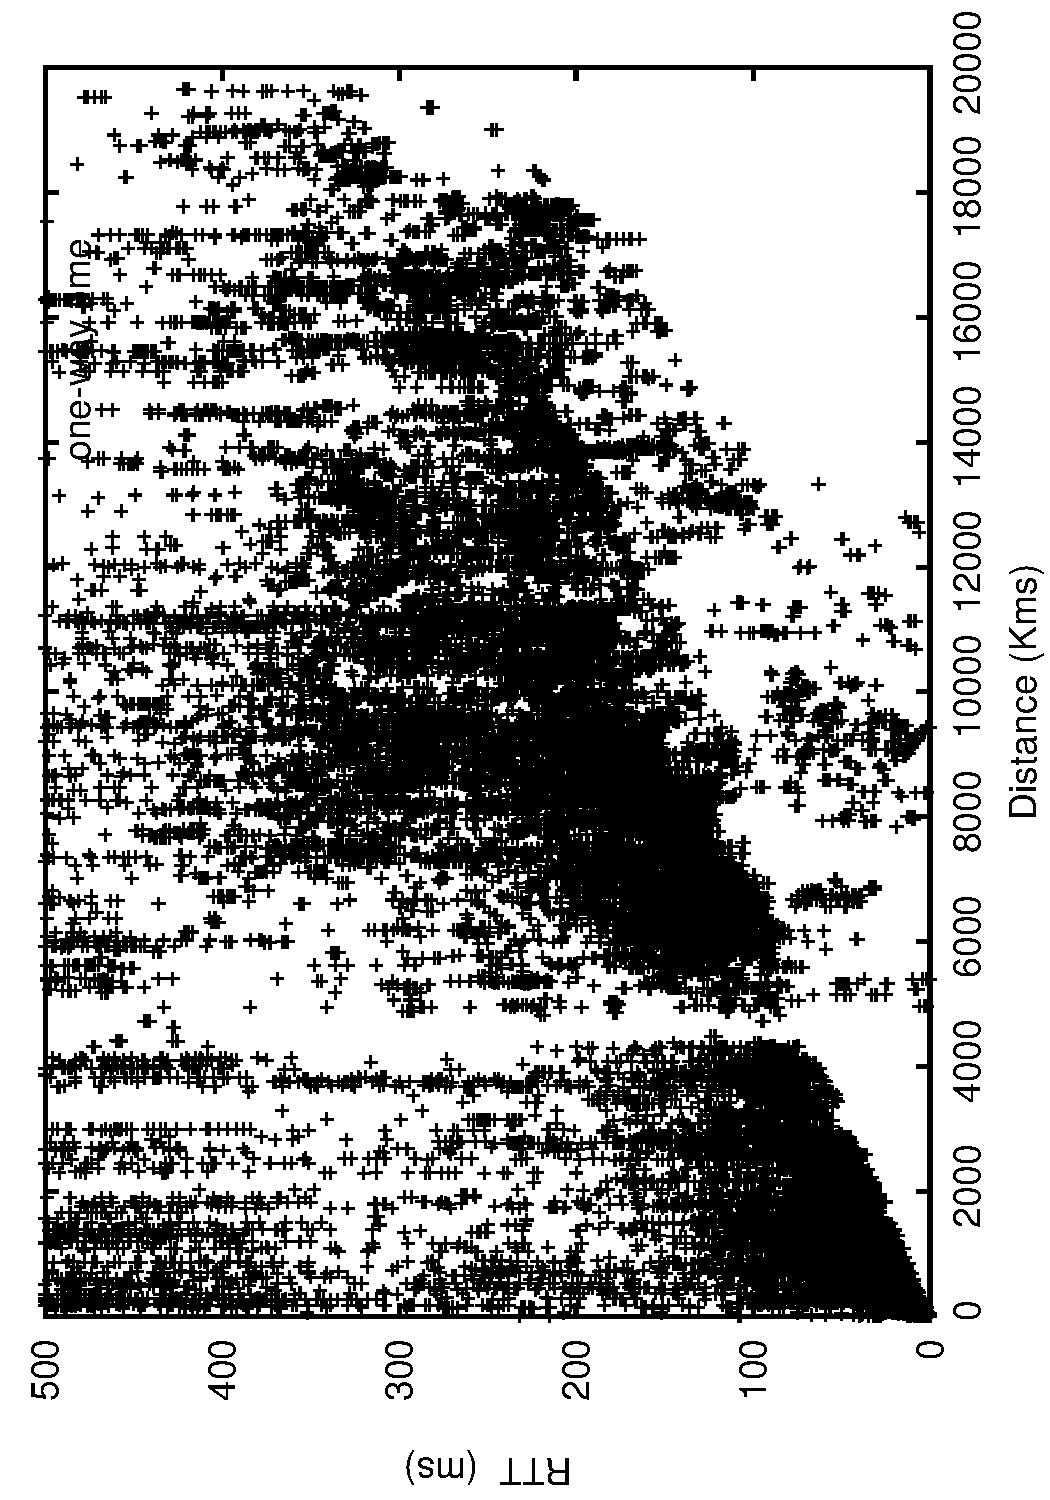
\includegraphics[width=2in,angle=270]{scatterplot_night.pdf}
\caption{My round-trip time measurements on Night data.}
\label{figure:scplt_night}
\end{figure}

\begin{figure}
\centering
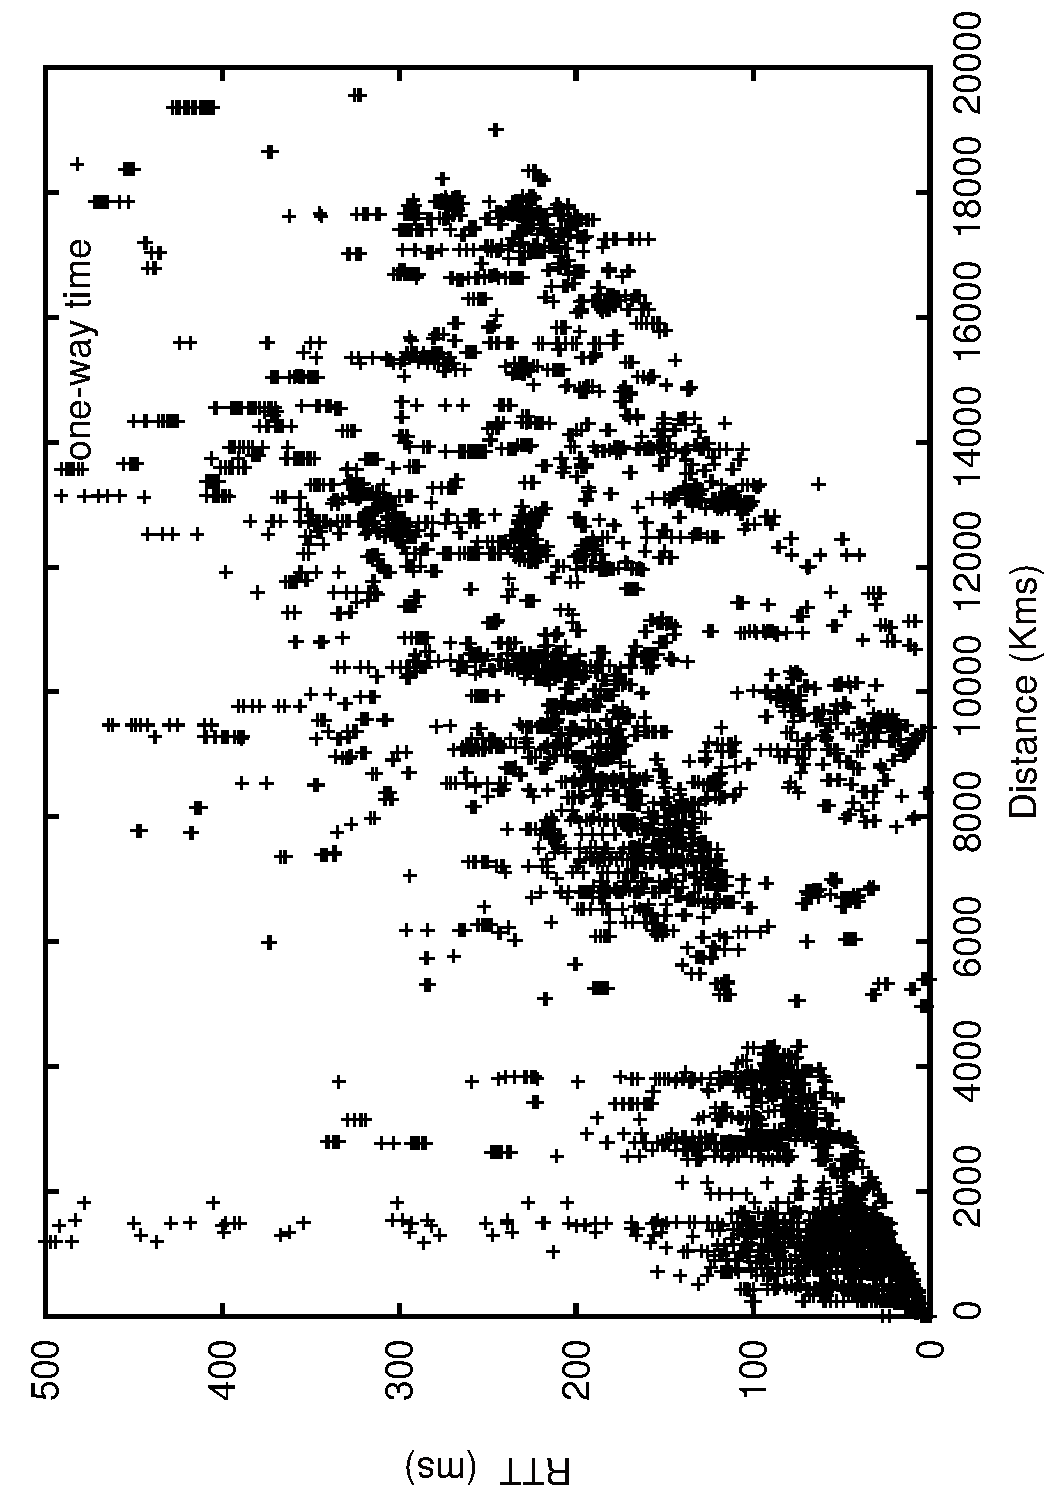
\includegraphics[width=2in,angle=270]{scatterplot_morning.pdf}
\caption{My round-trip time measurements on Morning data.}
\label{figure:scplt_morning}
\end{figure}

\begin{figure}
\centering
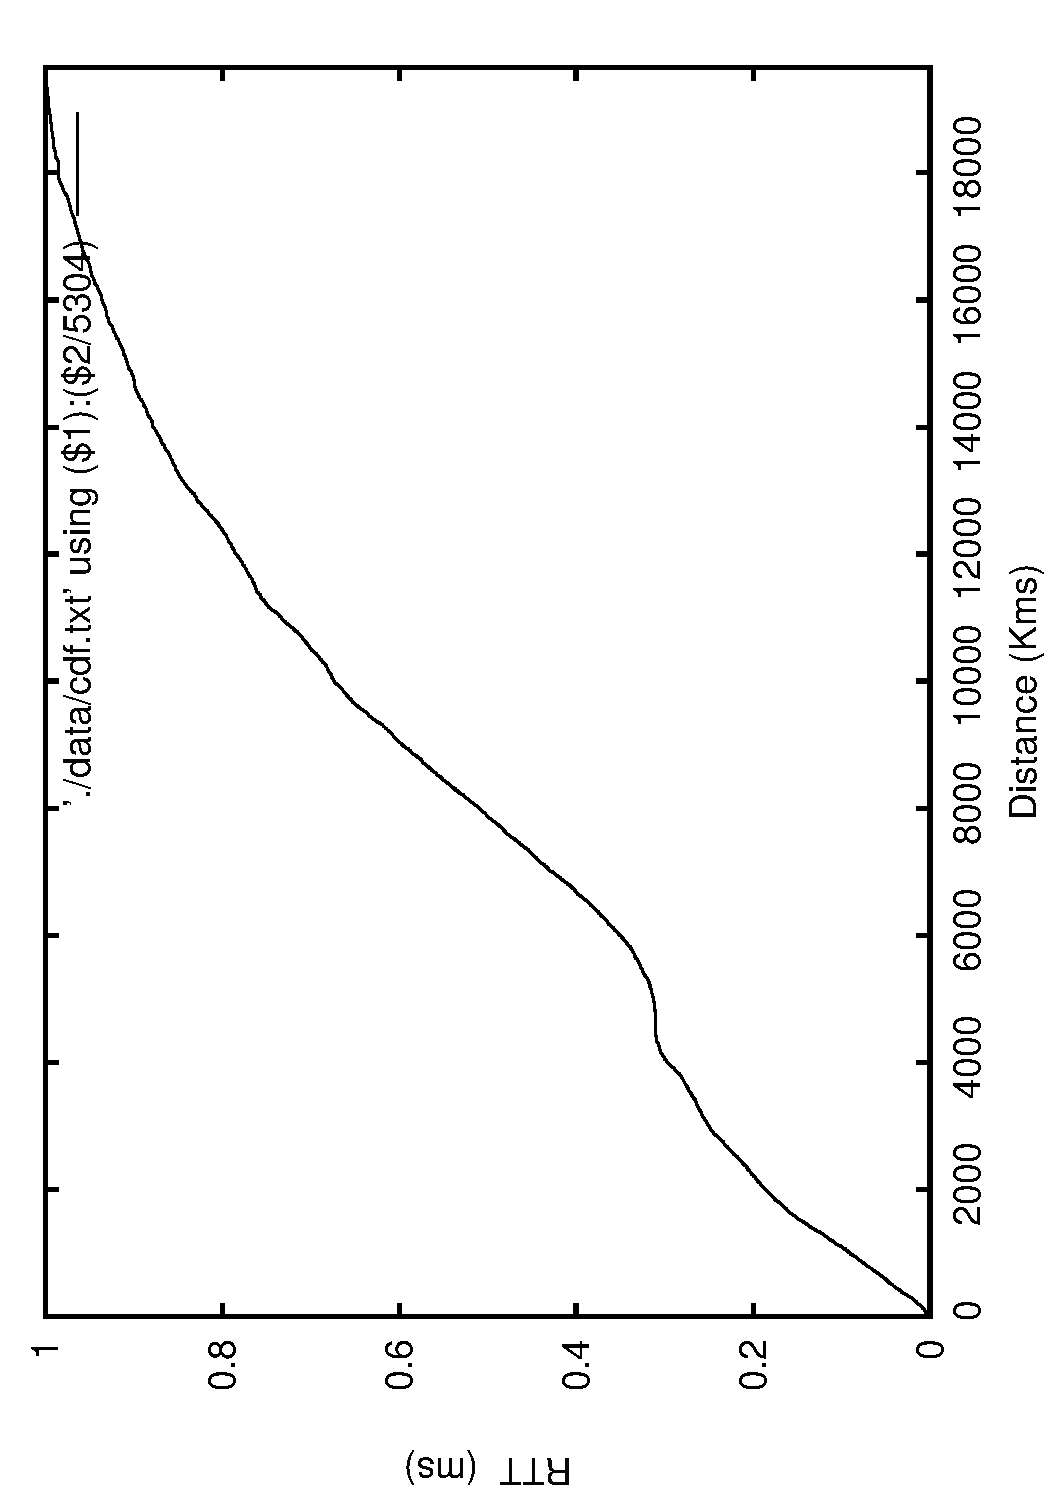
\includegraphics[width=2in,angle=270]{cdfplot_night.pdf}
\caption{My CDF plot on Night collected data.}
\label{figure:cdf_night}
\end{figure}

\begin{figure}
\centering
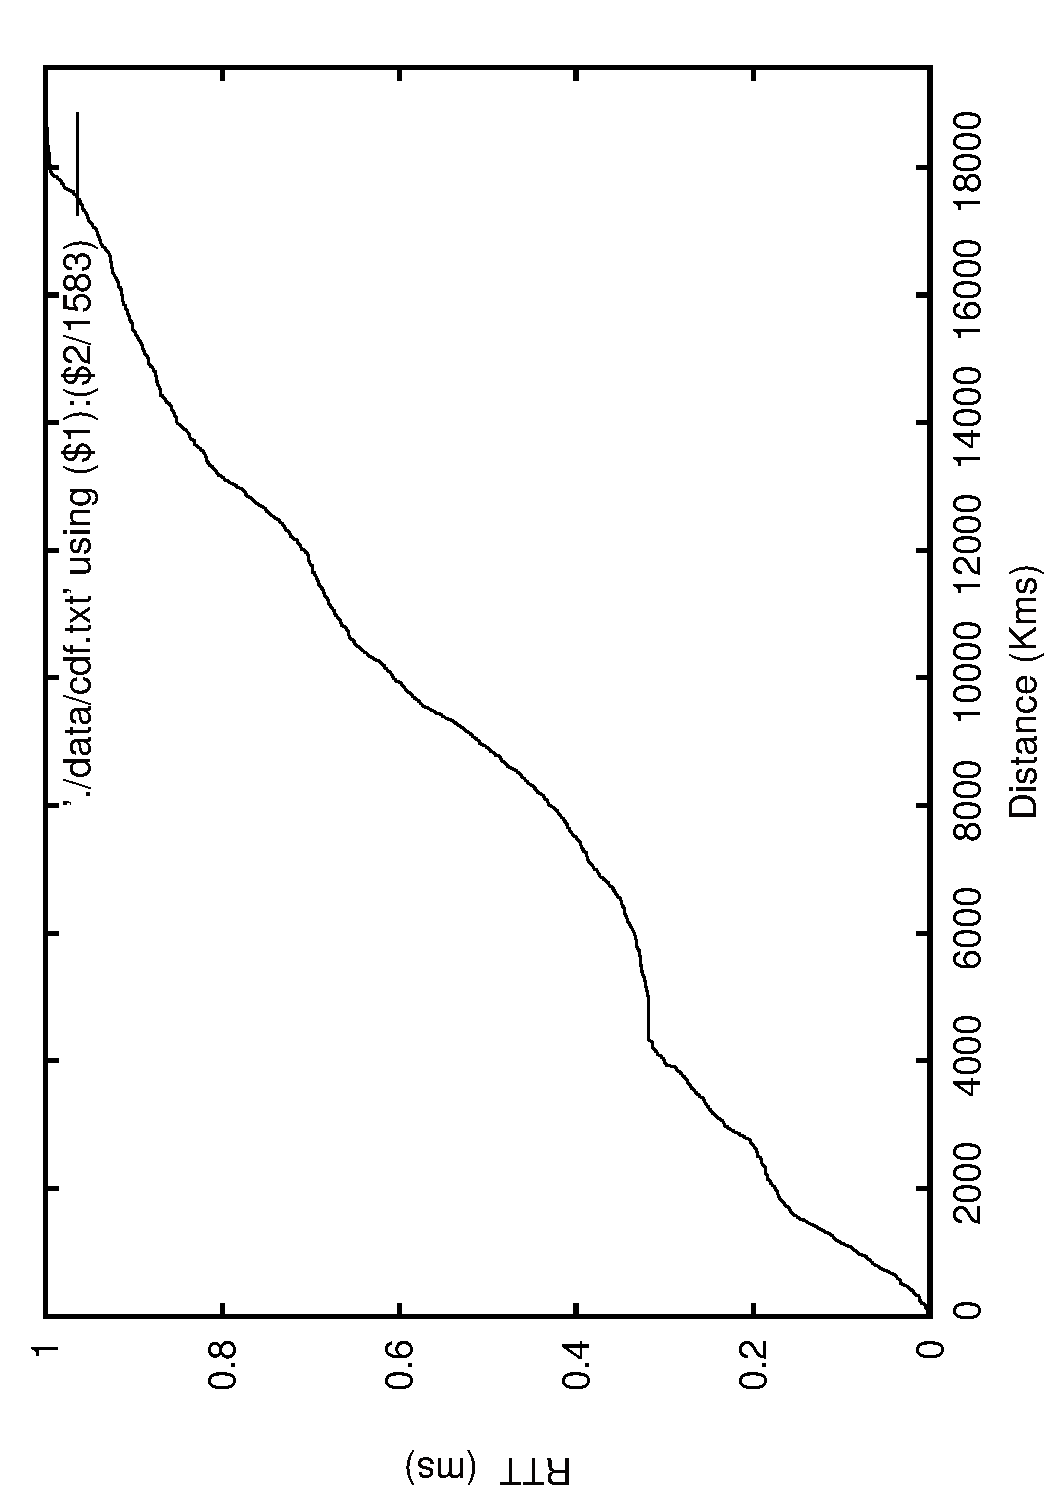
\includegraphics[width=2in,angle=270]{cdfplot_morning.pdf}
\caption{My CDF plot on Morning collected data}
\label{figure:cdf_morning}
\end{figure}

\begin{figure}
\centering
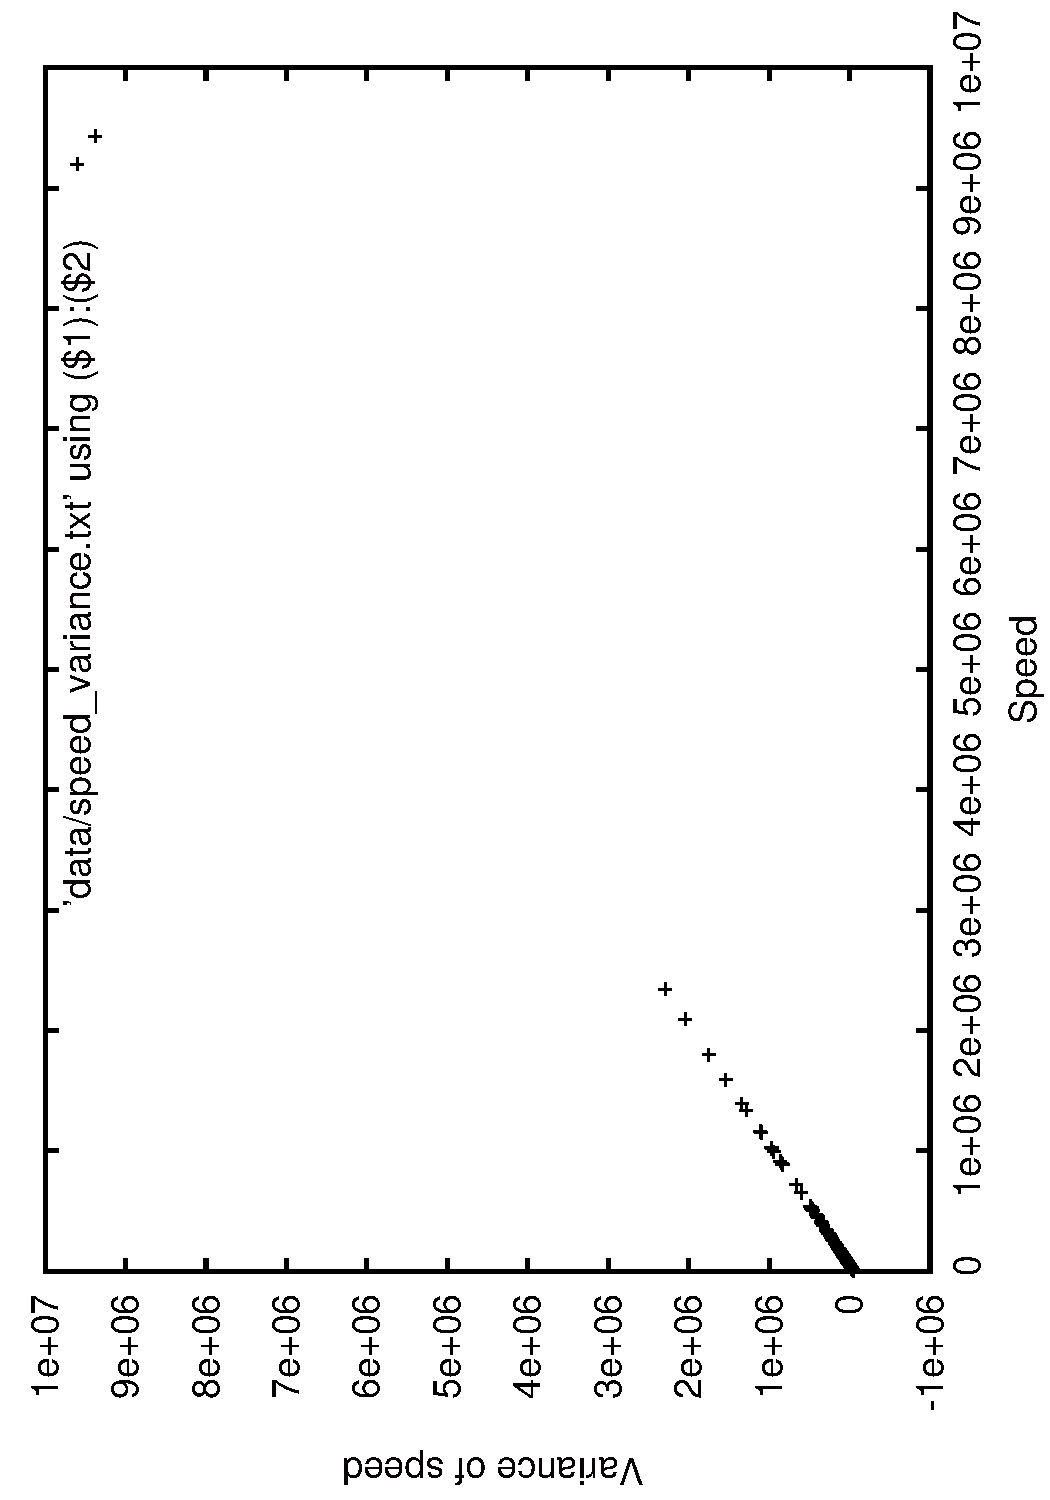
\includegraphics[width=2in,angle=270]{speed_sd_plot_night.pdf}
\caption{My SD plot on Night collected data}
\label{figure:sd_night}
\end{figure}

\begin{figure}
\centering
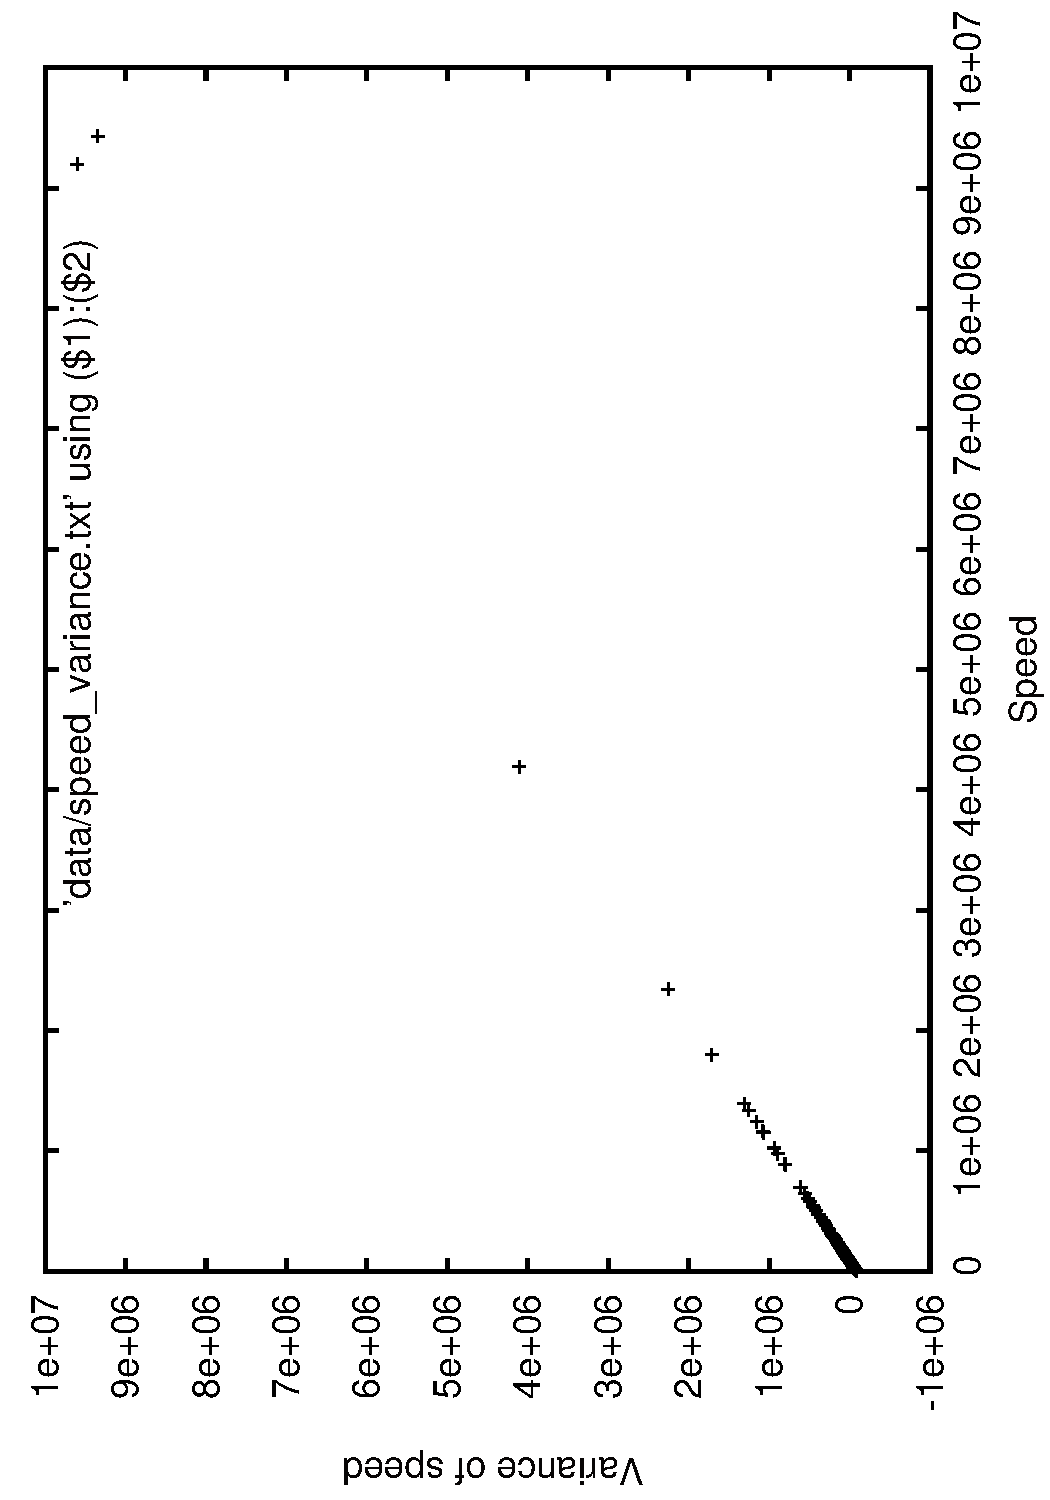
\includegraphics[width=2in,angle=270]{speed_sd_plot_morning.pdf}
\caption{My SD plot on Morning collected data}
\label{figure:sd_morning}
\end{figure}


\section{Analysis}

\subsection{Max. Speed of bits on internet}
Comparing to the maximum speed of light $$ {3*10^8 m/s} $$ the maximum speed of bits which I could infer from my dataset was maximum to the range of $$ {1*10^8 m/s} $$ which was below the speed of light it might be because of channel which carries the bits might be slow(bandwidth) or there might be many bottleneck connections which is shared among my channels.

\subsection{Poorly connected countries}
From the collected RTT dataset of all planet lab machines the \textit{To IP} address which always had the less ping time from all other machines is sorted out and the last few records are tailed, on looking at this data there are few IPs which are expected to be in the poorly connected countries. Few such IPs are listed below,
\begin{itemize}
\item 138.4.0.120
\item 130.216.1.22
\item 130.216.1.23
\item 163.117.253.23
\item 163.117.253.22
\item 156.62.231.242
\item 193.136.124.226
\item 202.112.28.100
\item 190.227.163.141
\end{itemize}

\subsection{Deducing IP location}
The IP address given for deduction \textit{68.86.95.9} is pinged from all the planet lab machines to all other machines, the RTT log is gathered out and this ping data is compared with the existing ping data set . The \textit{From IP, To IP, Distance, RRT} matching with the existing data pool is collated and by ball parking this is infered to be a location matching to IP \textit{128.252.19.18 with latitude 38.6479  and longitude -90.3015}

\section{Challenges}
There were few interesting challenges which I faced and almost succedded in solving them,
\begin{itemize}
\item To understand the awk, sed, many other bash commands and latex.
\item Spawning background jobs to expedite the process of collecting ping data.
\item Cleaning up the collected data and formatting them to process.
\item Sorting data based on various parameters and logically extracting them.
\item Understanding the math behind Standard Deviation, Cummulative Distribution and handling them.
\end{itemize}

\section{Conclusions}
This excerise on the whole helped me to understand the underneath concept of data travel around the internet, also a massive dataset was collected, cleaned and visualized with effective usage of shell scripting, few analysis was performed based on the dataset collected. 

\end{document}